% CVPR 2026 Paper Template; see https://github.com/cvpr-org/author-kit

\documentclass[10pt,twocolumn,letterpaper]{article}

%%%%%%%%% PAPER TYPE  - PLEASE UPDATE FOR FINAL VERSION
% \usepackage{cvpr}              % To produce the CAMERA-READY version
\usepackage[review]{cvpr}      % To produce the REVIEW version
% \usepackage[pagenumbers]{cvpr} % To force page numbers, e.g. for an arXiv version

% Import additional packages in the preamble file, before hyperref
\input{preamble}

% It is strongly recommended to use hyperref, especially for the review version.
% hyperref with option pagebackref eases the reviewers' job.
% Please disable hyperref *only* if you encounter grave issues, 
% e.g. with the file validation for the camera-ready version.
%
% If you comment hyperref and then uncomment it, you should delete *.aux before re-running LaTeX.
% (Or just hit 'q' on the first LaTeX run, let it finish, and you should be clear).
\definecolor{cvprblue}{rgb}{0.21,0.49,0.74}
\usepackage[pagebackref,breaklinks,colorlinks,allcolors=cvprblue]{hyperref}

%%%%%%%%% PAPER ID  - PLEASE UPDATE
\def\paperID{2022030173} % *** Enter the Paper ID here
\def\confName{GenAI Course}
\def\confYear{2026}

\toggletrue{cvprfinal}


%%%%%%%%% TITLE - PLEASE UPDATE
\title{Physics-inpired Quantum Error Mitigation by Generative Autoregression}

%%%%%%%%% AUTHORS - PLEASE UPDATE
\author{Panos Constantinides\\
School of Electrical and Computer Engineering, TU Crete\\
73100 Chania, Greece\\
{\tt\small pconstantinides.github.io}
}

\begin{document}
\maketitle
\begin{abstract}
Quantum error mitigation (QEM) is vital for achieving utility-scale quantum computing on noisy intermediate-scale quantum devices. While learning-based approaches offer flexible mitigation capabilities, traditional architectures often struggle to efficiently generalize across varying circuit depths and fail to explicitly decouple distinct noise processes. In this work, we present a novel, physics-informed generative framework for quantum error mitigation that specifically targets coherent noise accumulation. Our method introduces a probabilistic generative process that models local coherent errors as latent space representations of noise generators, which are subsequently propagated through a deterministic module derived from physical principles. This architecture extends the original Neural Noise Accumulation Surrogate (NNAS) framework proposed in \cite{xu2025} by incorporating structurally distinct surrogate branches for independent stochastic and coherent error tracking, alongside a regularized loss function that latent's distributions with the prior conditional one. To validate this framework, we developed the entire software pipeline from the ground up, encompassing the models, the training routines, and the mixed-noise synthetic dataset generation. Numerical evaluations provide proof-of-concept results showing that integrating a structured, physics-informed coherent branch successfully captures complex error characteristics without degrading the underlying stochastic mitigation performance of the surrogate framework, offering a principled foundation for more thorough research.
\end{abstract}    
\section{Introduction}
\label{sec:intro}

Quantum computing developes as a groundbreaking advancement that can tackle classicaly intractable probmels. 
Yet current hardware is limited both in terms of quality and quantity. Different error correcting codes have been proposed over the years that 
enable fault-tolerant quantum computation, yet such codes have been only demonstrated at small scales (Google Quantum AI and Collaborators 2024). Quantum error mitigation (QEM) can close this gap 
and enable utility scale quantum applications. The shared narative amongst QEM methods \cite{RevModPhys.95.045005} is governes between a trade-off between a moderate
resource overhead and a reduction of bias on the algorithms result, nevertheless QEM does not improve the quantum computer. On the other hand, the recent rise of generative models has demonstrated
that neural networks can capture complex patterns, especially in sequential task like text generation. In this work we model quantum processes as an autoregressive task, where noise is accumulated
at every layer. Upon that, a physics-inspired architecture is proposed that builds on the work by 

This work is structured in the following way
\section{Prior work}
\label{sec:prior_work}

%-------------------------------------------------------------------------
\subsection{Zero-Noise Extrapolation}
As discussed earlier, QEM methods rely on tractable increase in quantum resources along with additional classical processing.
Here we briefly describe zero-noise extrapolation \cite{PhysRevLett.119.180509,PhysRevX.7.021050} (ZNE) as a widely used method.
ZNE requires linear quantum runtime overhead combined with a classical extrapolation subroutine, making it atractive as a case agnaustic method.
To be more specific the ZNE approach is comprised of three steps: \textbf{(i)} Execute the target algorithm to obtain the scalar output,
\textbf{(ii)} execute theoretically equivalent versions of the algorithm but in a noisier setting, \textbf{(iii)} estimate the noiseless output by fitting a well-educated model.
These steps are showcased in Figure \ref{fig:zne} where noise amplification is achieved by global circuit folding, where the algorithm $U$ is uncomputed $U^\dagger$ and recomputed based on the unitary constraint
(see Appendix \ref{sec:computation}). This process effectively amplifies the noise while remaining theoretically equivalent to the original algorithm.

\begin{figure}
    \centering
    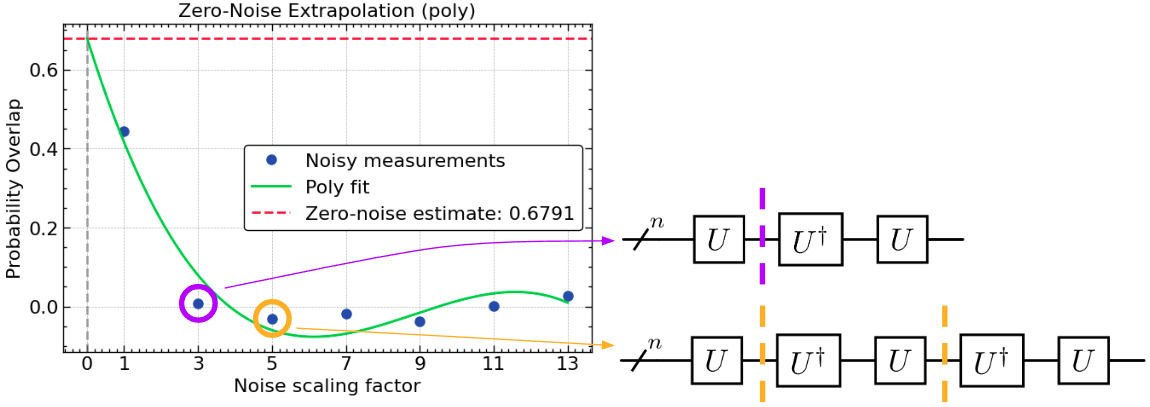
\includegraphics[width=\linewidth]{figures/zne.png}
    \caption{Error-mitigated estimate obtained using zero-noise extrapolation. Here extrapolation is performed using seven noisy data points.
    These are obtained by undoing $U^\dagger$ and redoing $U$ the quantum algorithm as many times as the scaling factor dectatets.}
    \label{fig:zne}
\end{figure}

Although ZNE is simple and powerful, it comes with some significant limitations. Firstly extrapolation is biased towards the rigid trend of the specified function, while it can be unstable when the noisy samples are similar.
Secondly granularity, noise drift.
It is also worth mentioning that using a neural network instead of function fitting is an active area of research.

%-------------------------------------------------------------------------
\subsection{The Neural Noise Accumulation Surrogate}
\label{sec:nnas-background}

Machine-learning approaches to quantum error mitigation (ML-QEM) typically treat the mapping from noisy to noiseless expectation values as an unstructured regression problem \cite{placidi2026deeplearningapproachesquantum}, learned from data produced by simulating or executing a circuit under a noise model. While such models can be effective at learning circuit features \cite{liao_machine_2024}, their black-box nature limits both their data efficiency and their ability to generalize across circuit depths.

The Neural Noise Accumulation Surrogate (NNAS) \cite{xu2025} addresses this by embedding a physical mechanisms directly into the network architecture. For a circuit of $L$ layers, NNAS models the noisy-to-noiseless mapping as a layer-wise sequential process, mirroring the way noise physically compounds as a circuit executes. Each noisy layer $\tilde{u}_l$ is decomposed via \emph{Maximum Noise Decomposition} (MND) into an ideal unitary $u_l$ composed with a stochastic, completely positive trace-preserving (CPTP) channel $\mathcal{E}_l$,
\begin{equation}
    \mathcal{E}_l = (1-p_l)\mathcal{I} + p_l \Lambda_l ,
\end{equation}
where $p_l$ is an empirically estimated effectiveness rate and $\Lambda_l$ is the residual CPTP channel (see also Appendix \ref{sec:errors}).
Propagating each layer's noise to the end of the circuit yields a cumulative noise envelope $R_l = \mathcal{U}_l \mathcal{N}_l \mathcal{U}_l^\dagger$, where $\mathcal{U}_l$ and $\mathcal{N}_l$ denote the circuit and noise channels respectively. The impact on the observable of interest is captured by a scalar impact factor $r_l$ via
\begin{equation}
    \text{Tr}[R_l\rho_l O] \rightarrow r_l\text{Tr}[\rho_l O]
\end{equation}
for a given target observable $O$.
As shown in \cite{xu2025} this yields the mitigated estimate
\begin{equation}
    y_l^{\mathrm{em}} = \frac{\tilde{y}_l}{\prod_{j=1}^{l}(1-\hat{p}_j) + \hat{r}_l} .
    \label{eq:mitigation}
\end{equation}
The first term in the denominator is a closed-form prior derived from the estimated effectiveness rates, the second term, $\hat{r}_l$, is the quantity NNAS is trained to predict. A schemantic representation of the autoregressive task is given by Figure \ref{fig:autoregressive_qem}.

\begin{figure}
    \centering
    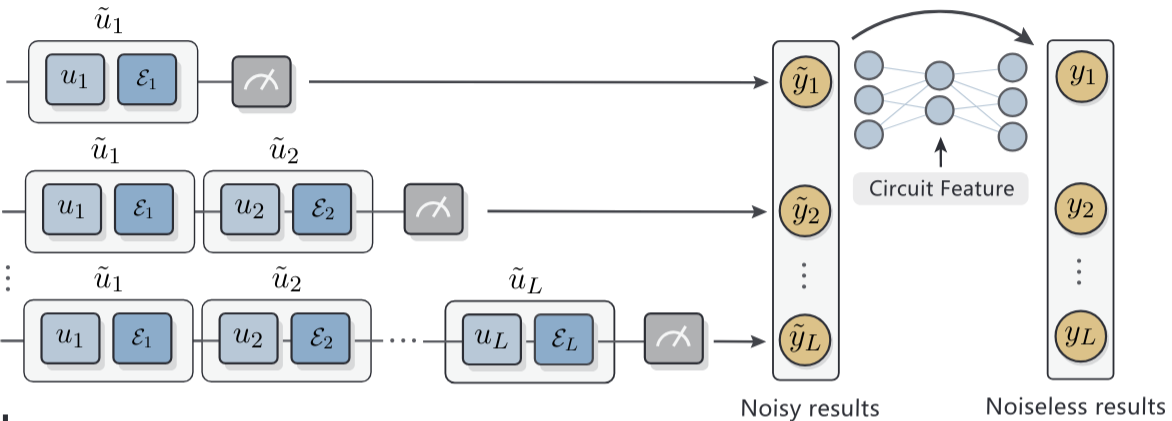
\includegraphics[width=\linewidth]{figures/autoregressive_qem.png}
    \caption{The illustration of layer-wise quantum sequential task. Figure adapted from \cite{xu2025}.}
    \label{fig:autoregressive_qem}
\end{figure}

Architecturally, NNAS instantiates this decomposition as a recurrent \emph{uniform neural accumulator}, a single hidden state $H_l$ updated as
\begin{equation}
    H_l = F(H_{l-1}, x_l),
\end{equation}
where $x_l$ embeds the circuit and device specification at layer $l$. This recursion mirrors the layer-by-layer composition of $\mathcal{U}_l$ and $\mathcal{N}_l$, so that $H_l$ implicitly represents the compressed state of noise accumulated up to layer $l$. Low-rank surrogates $\hat{\mathcal{U}}_l, \hat{\mathcal{N}}_l$ are recovered from $H_l$ via linear projections, and an attention mechanism,
\begin{equation}
    A_l = \mathrm{softmax}\!\left(\frac{\hat{\mathcal{U}}_l \hat{\mathcal{N}}_l^{T}}{\sqrt{d}}\right)\hat{\mathcal{U}}_l ,
\end{equation}
emulates the conjugate structure of $R_l = \mathcal{U}_l\mathcal{N}_l\mathcal{U}_l^\dagger$ before a final readout layer produces $\hat{r}_l$. Trained end-to-end against Eq.~\ref{eq:mitigation}, this design lets NNAS achieve strong mitigation accuracy from substantially less training data than unstructured regressors, and to degrade more slower with circuit depth, since the recurrent structure generalizes naturally to layer counts beyond those seen in training.

This efficiency, however, is inseparable from the specific physical assumption baked into the architecture: MND, and the effectiveness-rate prior it produces, is defined only for \emph{stochastic} CPTP channels. It has no representation for \emph{coherent} errors which act as unitary deviations rather than probabilistic mixtures. Such errors do not shrink the accumulated-noise prior $\prod_j(1-\hat p_j)$ toward zero in the way decoherence does. A single recurrent state $H_l$ trained under this architecture must therefore implicitly absorb both effects through the same update rule and the same scalar prior, with no structural signal distinguishing coherent noise.

In this work we extend the NNAS architecture by seperating the accumulation of noise into different branches for the two physically distinct error processes. A dedicated recurrent branch for coherent error accumulation is intriduced that is coupled to the existing stochastic branch and fused before the shared attention extractor.

\section{Methods}

\subsection{Physics-Informed Modeling of Coherent Errors}

The original NNAS architecture was developed to model errors due to decoherence through a recurrent latent representation (surrogates). Already it is shown \cite{xu2025} that NNAS outperforms a variaty of traditional QEM methods like ZNE. Nevertheless it does not explicitly capture coherent errors (for background see Appendix \ref{sec:errors}) arising from control imperfections or calibration drift.
These types of errors compose according to the algebra of unitary operators (see Appendix \ref{sec:computation}) and therefore exhibit noise accumulation that depends on the specific circuit and not so much the environment of the device. As a result, the original NNAS model is not designed to capture such errors.

To address this limitation, we upgrade NNAS with a seperate surrogate branch dedicated to coherent errors. This propagation mechanism is explicitly guided by physical principles. Rather than learning the evolution of coherent errors directly, the proposed architecture separates the estimation of local coherent error sources from their subsequent propagation. Specifically, each quantum circuit layer is associated with a latent coherent error generator,
\begin{equation}
    \label{eq:error_generator}
    \delta\mathbf{h}_l
\end{equation}
which represents the small unitary error introduced by the corresponding quantum gate. More specifically this is a purturbation to the ideal dynamics of the unitary operation, as described by Schrodinger's equation
\begin{equation}
    U_l^\text{noisy} = e^{i(\mathbf{H}_l + \delta\mathbf{h}_l)t}.
\end{equation}

Let $\Delta\mathbf{H}_{l-1}$ denote the accumulated coherent error generator after the $(l-1)$-th circuit layer. Given the ideal unitary operator $U_l$, the accumulated generator is updated according to

\begin{equation}
\Delta\mathbf{H}_l = \Delta\mathbf{H}_{l-1} + \mathrm{Ad}_{U_l}(\delta\mathbf{h}_l)
\end{equation}
where $\mathrm{Ad}_{U_l}(\cdot)$ denotes the adjoint action induced by the ideal gate. This first-order approximation transports each local generator into the global reference frame before accumulation. For applications requiring higher fidelity, the first Baker--Campbell--Hausdorff (BCH) correction can be incorporated,

\begin{equation}
    \Delta\mathbf{H}_l = \Delta\mathbf{H}_{l-1} + \mathrm{Ad}_{U_l}(\delta\mathbf{h}_l) + \frac{1}{2}
    \left[ \Delta\mathbf{H}_{l-1}, \mathrm{Ad}_{U_l}(\delta\mathbf{h}_l)\right]
\end{equation}
allowing the model to account for non-commuting coherent errors. Since this propagation module contains no trainable parameters, the evolution of coherent errors is purely physical. Consequently, the neural network is not required to learn coherent error composition and instead focuses exclusively on estimating local coherent error generators.

\subsection{Conditional Generation of Error Generators}

A central assumption of the proposed architecture is that coherent errors originate locally at individual circuit layers. Rather than directly predicting a global coherent error representation, the network learns a probabilistic model over these local error generators.
At every circuit layer $l$, a recurrent neural network receives the embedded circuit representation $\mathbf{x}_l$, the gate descriptor $\mathbf{g}_l$, and the previous hidden state. The recurrent representation is used to parameterize a conditional Gaussian posterior

\begin{equation}
    q(\delta\mathbf{h}_l|\mathbf{x}_l,\mathbf{g}_l) = \mathcal{N}(\boldsymbol{\mu}_l,\mathbf{\Sigma}_l)
\end{equation}
whose latent variable corresponds to the coherent error generator as in Eq. \ref{eq:error_generator}. Samples are obtained using the standard reparameterization trick,

\begin{equation}
    \delta\mathbf{h}_l = \boldsymbol{\mu}_l + \boldsymbol{\sigma}_l \odot \boldsymbol{\epsilon}
    \text{  with  }
    \boldsymbol{\epsilon} \sim \mathcal{N}(\mathbf{0}, \mathbf{I})
\end{equation}
which makes the sampling process differentiable.

The key intuition behind the generative task is that coherent errors are not deterministic quantities but depend on multiple unobserved factors, including calibration uncertainty, control electronics, and environmental fluctuations. Modeling coherent error generators as latent random variables therefore provides a proper mechanism for representing uncertainty while allowing the network to learn distributions rather than single deterministic values.
Furthermore, different quantum gates exhibit distinct coherent error characteristics. For example, single-qubit rotations and two-qubit entangling gates are typically subject to noise levels. To encode this prior knowledge, we introduce a gate-conditioned prior network,

\begin{equation}
    p(\delta\mathbf{h}_l|\mathbf{g}_l) = \mathcal{N}
    (\boldsymbol{\mu}^\text{prior}_l, \mathbf{\Sigma}^\text{prior}_l)
\end{equation}
implemented as a lightweight multilayer perceptron that receives only the gate descriptor as input. This prior captures the expected statistics of coherent error generators for each gate type while remaining independent of the surrounding circuit context. During training, the inferred posterior is encouraged to remain close to this physically motivated prior, allowing circuit-specific coherent errors to be learned without discarding prior information about gate-dependent error behavior.


\subsection{Model Fusion and Training}

The coherent and incoherent branches evolve independently throughout the architecture. The later follows the original NNAS formulation and models the accumulation of incoherent noise using its recurrent surrogate representation. In parallel, the proposed coherent branch generates local coherent error generators and propagates them through the deterministic algebraic module described above.
After propagating the coherent generators, the accumulated coherent representation $\Delta\mathbf{H}_l$ is projected into the latent feature space through a linear projection layer. This projected representation is concatenated with the stochastic latent representation produced by the original NNAS branch before being processed by the existing neural extractor. Consequently, the final attention-based module simultaneously receives information describing both incoherent and coherent error processes as an extensions to the original NNAS architecture.

The model is trained end-to-end using the original mitigation MSE objective supplemented by a Kullback--Leibler regularization term,

\begin{equation}
    \mathcal{L} = \mathcal{L}_{\mathrm{mitigation}}
    +
    \beta D_{\mathrm{KL}}\left(q(\delta\mathbf{h}_l|\mathbf{x}_l,\mathbf{g}_l)\;\|\;p(\delta\mathbf{h}_l|\mathbf{g}_l)\right)    
\end{equation}
where $\beta$ controls the contribution of the latent regularization. The mitigation loss remains unchanged from the original NNAS formulation, while the KL divergence regularizes the inferred coherent error generators toward the gate-conditioned prior. This objective encourages the network to generate coherent error distributions that are both physically plausible and informative for the mitigation task.

Training is performed using the same circuit dataset employed by the original NNAS. To evaluate the proposed extension, the dataset is augmented with synthetic coherent noise by introducing systematic over-rotations and gate-dependent calibration offsets in addition to the existing noise models. Mixed-noise datasets are generated by combining coherent and incoherent error channels, enabling the model to learn realistic hardware noise characteristics. The proposed architecture is trained under the same optimization settings as the original NNAS, allowing improvements in mitigation performance to be attributed solely to the incorporation of the physics-informed coherent error branch while leaving room for future work.

\section{Results}

The primary objective of this study is to establish the feasibility of the proposed physics-informed extension of NNAS rather than to optimize its predictive performance. Consequently, the experiments presented in this section should be viewed as a proof-of-concept evaluation designed to assess whether the proposed architecture can successfully integrate physically motivated coherent error modeling while maintaining the mitigation capabilities of the original NNAS. A comprehensive exploration of hyperparameter optimization, larger-scale datasets, and study of more accurate prior distributions is left for future work.

To evaluate the proposed extension, we compare the original NNAS architecture with four different models: (i) the original NNAS, (ii) a dual-state architecture combining stochastic and coherent branches, (iii) stochastic-only and coherent-only versions and (iv) the proposed physics-informed generative model. Performance is reported in terms of mean absolute error (MAE) as a function of circuit depth under four noise settings: stochastic, coherent, mixed, and coherent drift. The noisy (unmitigated) baseline is included for reference.

\begin{figure*}[t]
    \centering
    
\includegraphics[width=\textwidth]{figures/error_vs_depth_3.png}
    \caption{Mean absolute error (MAE) as a function of circuit depth for the original NNAS, the proposed physics-informed generative extension as well as it's non generative (dual state) version and baseline variants under stochastic, coherent, mixed, and coherent drift noise models. All learned approaches demonstrate some error mitigation potential the unmitigated baseline, while the proposed method achieves mitigation performance comparable to existing NNAS variants across all evaluated noise settings.}
    \label{fig:results}
\end{figure*}

\subsection{Stochastic Noise}

Figure~\ref{fig:results} (upper left) shows the mitigation performance under purely stochastic noise. All learned models substantially outperform the unmitigated baseline across the entire depth range, demonstrating that the proposed coherent modeling does not degrade the stochastic mitigation capabilities inherited from the original NNAS. The proposed dual-state architecture achieves the lowest MAE (no generative part) for most circuit depths, while the physics-informed generative model remains competitive, exhibiting only a modest increase in prediction error at larger depths. As expected, the stochastic-only model performs comparably to the original NNAS. These observations suggest that the additional coherent branch does not interfere with the stochastic representation learned by the original architecture.

\subsection{Coherent Noise}

The coherent noise experiment is shown in Fig.~\ref{fig:results} (upper right). Under the current experimental configuration, all coherent-aware architectures exhibit comparable performance across the evaluated circuit depths, with no approach consistently outperforming the others. Although the proposed physics-informed generative model does not provide a measurable improvement in mitigation accuracy for this proof-of-concept setting, it demonstrates that explicitly modeling coherent error generators through a probabilistic latent representation and deterministic algebraic propagation can be incorporated into the NNAS framework without degrading performance.

\subsection{Mixed Noise}

Results under simultaneous stochastic and coherent noise are shown in Fig.~\ref{fig:results} (lower left). The proposed model maintains performance comparable to the competing architectures throughout the evaluated depth range. While no single model consistently dominates, the physics-informed generative branch exhibits stable behavior as circuit depth increases and remains significantly below the unmitigated error. This indicates that separating stochastic and coherent latent representations allows the network to model both error sources simultaneously without sacrificing predictive performance.

\subsection{Coherent Drift}

Results under coherent drift are presented in Fig.~\ref{fig:results} (lower right). Similar to the coherent-only experiment, all learned models achieve comparable mitigation performance throughout the evaluated depth range, and no consistent performance advantage is observed for any particular architecture. These results suggest that, under the current dataset and model configuration, the proposed coherent branch performs on par with existing approaches while introducing a physically motivated and interpretable representation of coherent error propagation.

Overall, the proposed physics-informed generative extension achieves mitigation performance comparable to that of the original NNAS and the dual-state (non generative) baseline across all evaluated noise models. While the present proof-of-concept does not demonstrate a consistent reduction in MAE over existing approaches, it shows that incorporating explicit physical structure into the coherent branch does not compromise predictive accuracy. More importantly, the proposed formulation introduces an interpretable decomposition in which local coherent error generators are inferred probabilistically and propagated according to a deterministic mathematical model, providing a principled foundation for future extensions involving more accurate coherent error propagation and hardware-informed priors.

\section{Conclusion}

In this work, we proposed a physics-informed extension of the Neural Noise Accumulator and Suppressor (NNAS) architecture for learning-based quantum error mitigation. Unlike the original formulation, which models noise accumulation using purely data-driven recurrent dynamics, the proposed approach explicitly distinguishes between stochastic and coherent error processes. Local coherent error generators are modeled probabilistically through a conditional latent-variable model and propagated using a deterministic model derived from the Baker--Campbell--Hausdorff expansion. This decouples the estimation of coherent error sources from their physical evolution, yielding a more interpretable and physical architecture.

The experimental results presented in this work serve as an initial proof of concept. Although the proposed model does not consistently outperform existing NNAS variants under the current datasets and experimental configurations, it demonstrates that physics-informed coherent error modeling can be integrated into a learning-based error mitigation framework without sacrificing predictive performance. More importantly, the proposed formulation establishes a new direction for combining generative machine learning with physically constrained models of quantum noise.

The principal contributions of this work are summarized as follows:

\begin{itemize}
    \item We propose a physics-informed extension of the NNAS architecture for coherent error mitigation.
    \item We introduce a conditional generative model for learning local coherent error generators.
    \item We incorporate deterministic propagation into the coherent branch, inspired by the BCH decomposition .
    \item We demonstrate proof-of-concept results, showcasing that this work can be integrated into NNAS without degrading mitigation performance.
\end{itemize}

\subsection*{Future Work}

Future work will focus on imporving the training pipeline as well as gate-conditioned priors. Also evaluation on larger datasets and real quantum hardware are prominent directions.

\section*{Implementation availability}
The code, datasets and trained models have been made temporarily open source \cite{github} as this work is still in progress.

{
    \small
    \bibliographystyle{ieeenat_fullname}
    \bibliography{main.bib}
}
\clearpage
% \setcounter{page}{1}
% \maketitlesupplementary

\appendix
\section{Practical quantum copmutation}
The purpose of this section is to provide the reader with the minimal understanding of quantum information, processes and errors.
Although quantum computation lives in Hilbert space, for this appendix we will omit that by assuming the space of complex numbers.
Readers familiar with quantum computation may skip this part.

\subsection{Information}
Quantum systems that are subject to noise are described by a density operator, which is represented as a matrix.
\begin{definition} (density matrix - loose)
The density matrix $\rho\in\mathbb{C}^{2^n\times 2^n}$ decsribing a $n$-qubit system is positive semi-definite with unit trace.
That is, for every eigenvalue $\lambda_i$ of $\rho$: $\lambda_i\in\mathbb{R}$ and $\lambda_i\geq 0$ with $\sum_i \lambda_i=1.$
\end{definition}

\noindent Additionally when a state $\rho$ is coupled with the environment is called \textit{mixed}, otherwise is refered to as \textit{pure} and it satisfies $\rho^2=\rho$ (i.e. a projector).

At this point it should be obvious that a full-state simulation of a quantum system is difficult due to the exponential scaling of the state.
Nevertheless, there are thechniques that \cite{waintal2026competequantumcomputerslecture,PhysRevLett.128.220503} are efficient in regimes with low correlations.

\subsection{Computation}
\label{sec:computation}
Computation is realized through quantum processes, which in the ideal case are unitary maps

\begin{definition} (unitary process)
\label{def:unitary}
A $n$-qubit state $\rho$ is evolved under the unitary transformation as
\begin{equation}
    \mathcal{U}(\rho) = U\rho U^\dagger
\end{equation}
where $U\in\mathbb{C}^{2^n\times 2^n}$ with $U^{-1}=U^\dagger$ and $\cdot^\dagger$ denoting the conjugate-transpose.
\end{definition}

In practise, such processes couple the system with the environment leading to loss of coherence withing the computational states.
Such noisy processes (or channels) are captured by completely-positive and trace preserving (CPTP) maps. Which in the so called Stinespring representation
are described as follows.

\begin{definition} (quantum channel)
\label{def:channel}
A quantum channel $\mathcal{E}$ acting on some $n$-qubit state $\rho$ is defined as
\begin{equation}
    \mathcal{E}(\rho) = \sum_i p_i K_i\rho K_i^\dagger
\end{equation}
the matrices $K_i$ are known Krauss operators and satisfy the completness relation
\begin{equation}
    \sum_i K_i K_i^\dagger = I_{2^n}.
\end{equation}
\end{definition}

\subsection{Quantum errors}
\label{sec:errors}

Since the subject of this work is to mitigate quantum errors, it is appropriate to give some additional background.
Quantum errors can be classified in two main classes: coherent and incoherent errors. Firstly, coherent errors arise due to
imperfections in the quantum control modules of the processor. These are typically quantified by gate fidelity metrics and
the current state-of-the-art ranges from 99-99.99\% for two-qubit gates. These are considered the dominant source of errors.
Such errors are described by imperfections in unitary operations (see Def. \ref{def:unitary}).
Secondly, incoherent noise arises once the system gets coupled with the environment, and are formulated as quantum channels.

The maximum noise decomposition (MND) is an abstract way of describing decoherence, where different noise channels are aggregated under one error rate
\begin{equation}
    \mathcal{E} = (1-p)\mathcal{I} + p \Lambda
\end{equation}
where $\Lambda$ is the effective (aggregated) noise channel and $\mathcal{I}$ is the identity channel. We will refer to $p$ as the effective error rate.

\section{Flowchart of the architecture}
\begin{figure*}
    \centering
    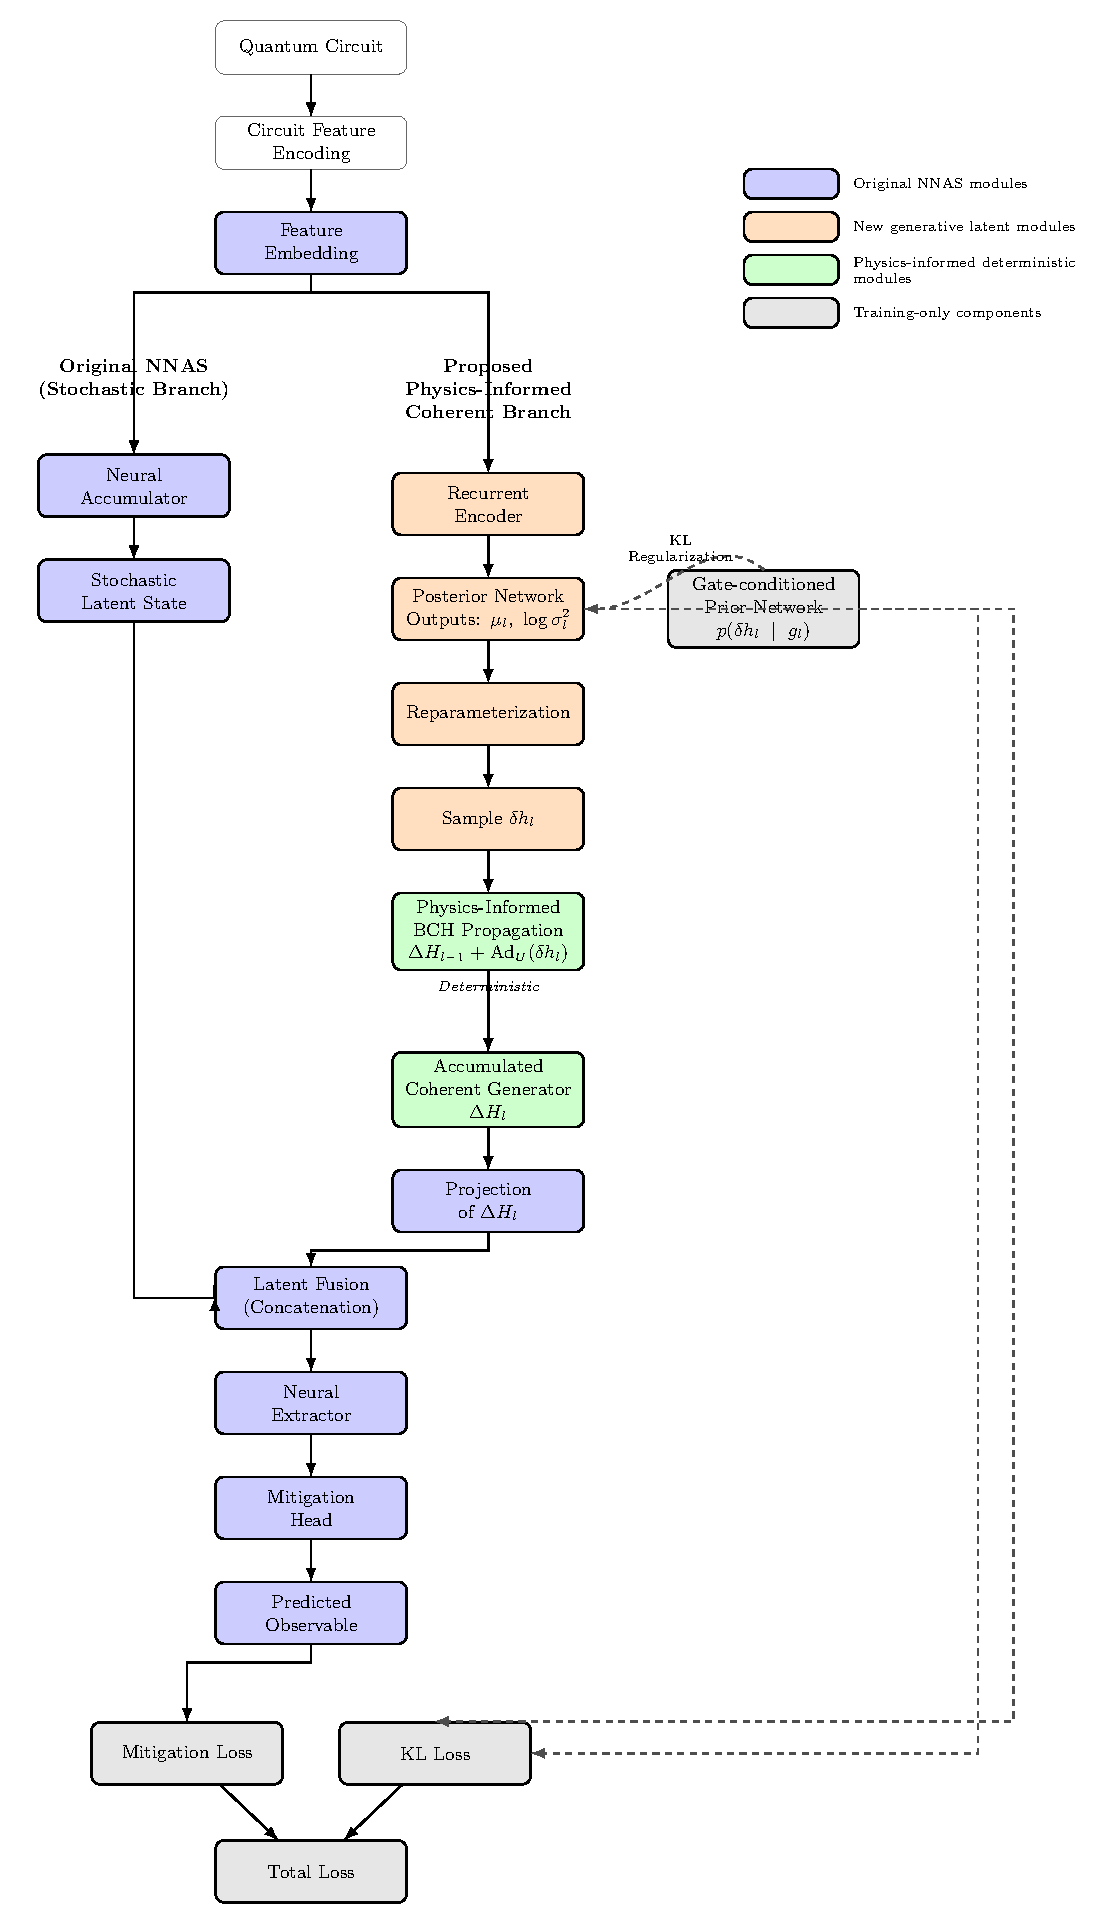
\includegraphics[scale=0.62]{flowchart.pdf}
    \caption{Proposed extension of the NNAS architecture. The original stochastic branch is preserved, while a new conditional generative coherent branch estimates local coherent error generators. These generators are propagated through a deterministic BCH-inspired module before being fused with the stochastic latent representation. During training, a gate-conditioned prior regularizes the latent coherent generators through a Kullback--Leibler divergence, while inference relies solely on the learned posterior and the physics-informed propagation module.}
    \label{fig:nnas-architecture}
\end{figure*}

\end{document}
